\chapter{Object Detection Using Exemplar Models} % (fold)
\label{cha:object_detection}

Because NBNN classification uses individual descriptors, it seems natural to look for a detection method that uses these descriptors directly, when you want to adapt NBNN to detection. Exemplar models do just that, and have been used in similar attempts before \cite{becker2012codebook}.

\section{Exemplar Models} % (fold)
\label{sub:exemplar_models}

Exemplar models \cite{leibe2004combined, chum2007exemplar} are related to part-based models. In exemplar model detection, for each object feature found during training, an exemplar is stored. The exemplar represents the size and location of the bounding box relative to the feature. The exemplars are aggregated into part models \cite{leibe2004combined} or visual words \cite{chum2007exemplar}. In this way a class is modeled by a set of exemplars that have a high probability of occurring in a certain location and at a certain scale of the image.

At test time, each feature found in the test image is matched with the exemplars stored, and from this combination of the location and scale of the feature found, and the exemplar it is matched with, a hypothesis can be formed for the object's location in the test image. This means that each feature in the test image gets a vote, weighted by the quality of its match, for a bounding box. These hypotheses can be clustered into detection windows (See Figure~\ref{fig:exemplar_model}). Experiments show that this method performs well too as a first step in a cascade setting. \cite{vedaldi2009multiple}

\begin{figure}[hbt]
    \centering
    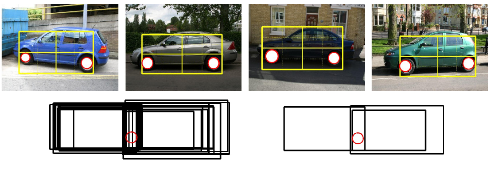
\includegraphics[width=0.9\textwidth]{ExemplarModel}
    \caption{Given four images of car sides, their bounding boxes (yellow) and 8 features of a car wheel (above), for each feature an exemplar is made, where its position and size relative to the bounding box is used. So when a feature is found during test time, that is similar to a car wheel, a number of hypotheses is formed by applying the exemplars to the new feature (below left, in black). These hypotheses can be clustered into a small amount of highly likely detections. (Taken from Chum and Zisserman \cite{chum2007exemplar}.)}
    \label{fig:exemplar_model}
\end{figure}

% subsection exemplar_models (end)

\section{Clustering Algorithms} % (fold)
\label{sub:clustering_algorithms}

In exemplar-model detection, hypotheses of bounding boxes need to be clustered into detections. These detections represent the classes, which are inherently unknown, and depend fully on the image at hand, and the hypotheses that have been derived from it. The number of objects in the image is unknown, so the number of clusters should not be fixed.

K-means clustering is a well known clustering algorithm. It divides all objects in a pre-defined number of $k$ clusters, minimizing the sum of squared distances of all objects within each separate cluster. An important reason why it is not appropriate for this task, is that we do not have an indication of the number of clusters we want. Therefore, other algorithms have to be considered.

\begin{figure}[hbt]
    % \centering
    \begin{subfigure}[b]{0.32\textwidth}
            \centering
            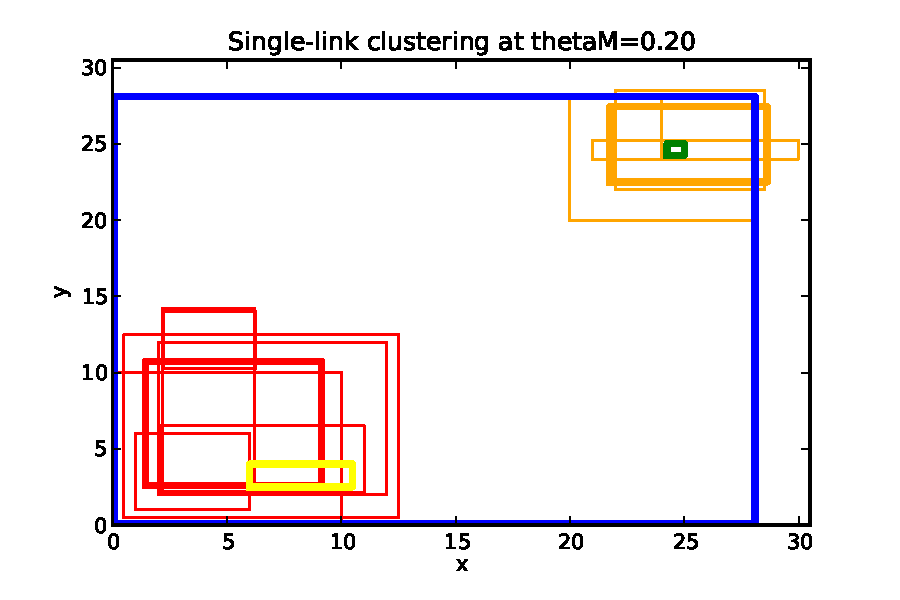
\includegraphics[width=\textwidth]{visSL020}
            \caption{}
            \label{fig:slvqs_qs1}
    \end{subfigure}
    ~ %add desired spacing between images, e. g. ~, \quad, \qquad etc.
      %(or a blank line to force the subfigure onto a new line)
    \begin{subfigure}[b]{0.32\textwidth}
            \centering
            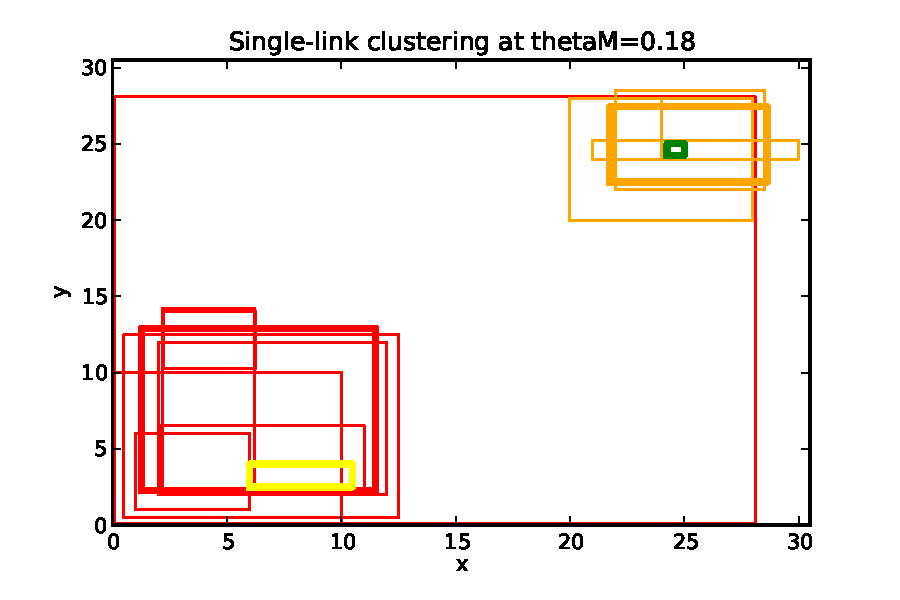
\includegraphics[width=\textwidth]{visSL018}
            \caption{}
            \label{fig:slvqs_qs2}
    \end{subfigure}
    ~ %add desired spacing between images, e. g. ~, \quad, \qquad etc.
      %(or a blank line to force the subfigure onto a new line)
    \begin{subfigure}[b]{0.32\textwidth}
        \centering
        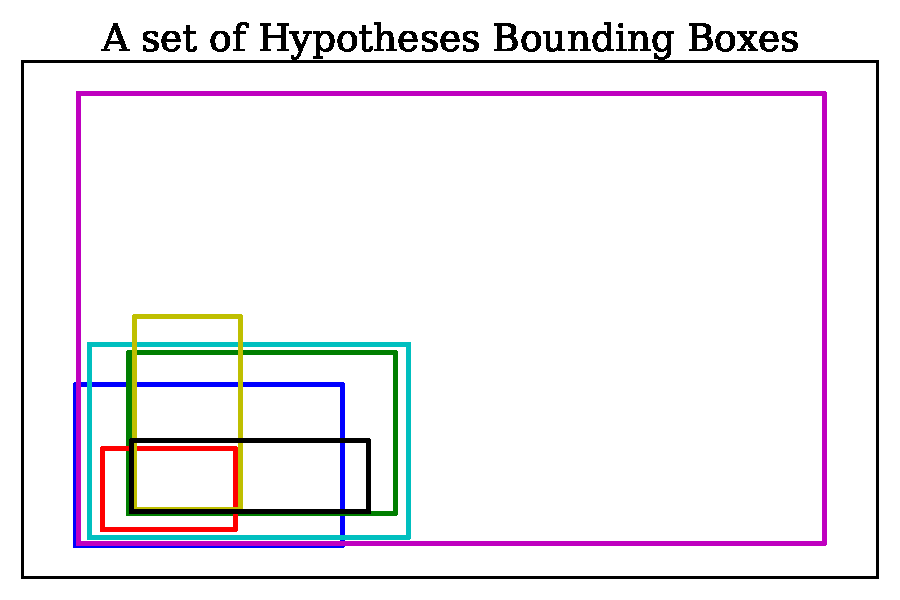
\includegraphics[width=\textwidth]{visBB}
        \caption{The set of hypotheses.}
        \label{fig:slvqs_bb}
    \end{subfigure}%

    \begin{subfigure}[b]{0.32\textwidth}
            \centering
            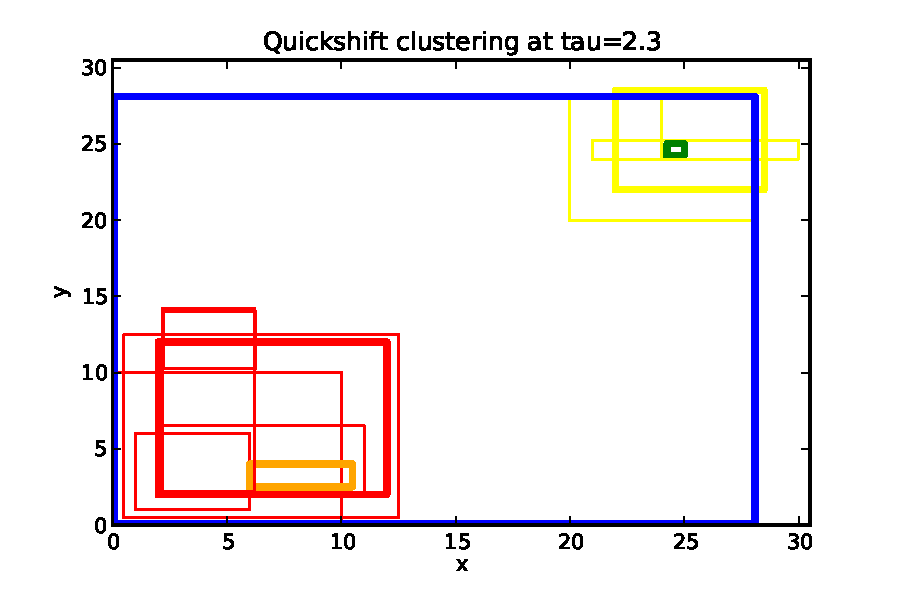
\includegraphics[width=\textwidth]{visQS23}
            \caption{}
            \label{fig:slvqs_sl1}
    \end{subfigure}
    ~
    \begin{subfigure}[b]{0.32\textwidth}
            \centering
            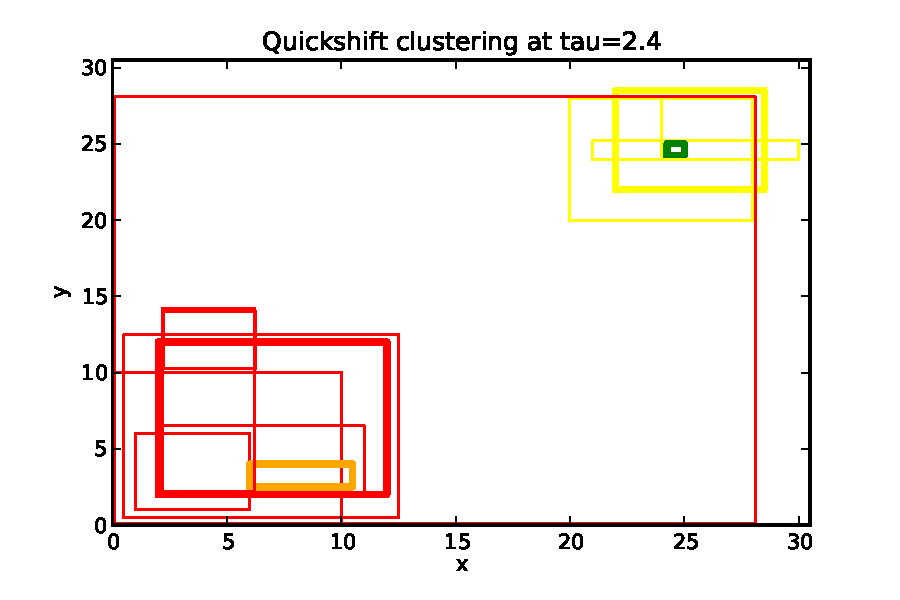
\includegraphics[width=\textwidth]{visQS24}
            \caption{}
            \label{fig:slvqs_sl2}
    \end{subfigure}
    \caption{The main difference between agglomerative clustering as used by Becker, and quickshift clustering is the way the detection is determined from the cluster. In single-link clustering, the inclusion of a single hypothesis into a cluster can have a large effect on the detection formed from this cluster: The blue hypothesis in (a) is included in the red cluster (b), making the red detection (bold line) almost twice as big. Using quickshift (d,e) this inclusion does not have any effect on the detection itself, because the local maximum of the red cluster is unchanged.}
    \label{fig:sl_vs_qs_clustering}
\end{figure}

\subsection{Agglomerative Clustering} % (fold)
\label{sub:agglomerative_clustering}

It is possible to view a clustering clustering algorithm as a tree, where the leaves represent the objects to be clustered. If the pairwise distances between all objects are known, the leaves can be joined into clusters iteratively, each time merging the two closest objects into a cluster. When these clusters are clustered again based on distance, merging will continue until there is only one single cluster left. Afterwards, this tree could be split into clusters by cutting branches that exceed a certain threshold distance, $\theta_m$. This clustering algorithm is called agglomerative clustering. It is a subtype of hierarchical clustering, other hierarchical algorithms not being agglomerative, but divisive, starting with one single cluster.

There is some variety in the ways to merge leaves into clusters. Single link clustering means that the minimum distance between members of each cluster is the basis of further clustering, complete linkage and mean linkage clustering take the maximum distance and the mean distance, respectively.

When clustering hypotheses, a substantial part of clustering consists of defining a detection from a cluster of hypotheses. In agglomerative clustering this is not clearly defined, because, even though there is a hierarchy in clustering, it does not follow from the algorithm where the cluster center is located. Therefore, the values of cluster members are averaged to find a detection. \cite{becker2012codebook} In a Euclidean clustering space, this is a reasonable approach, even though there is no theoretical reason to do it this way.

% subsubsection agglomerative_clustering (end)

\subsection{Mode-finding Algorithms} % (fold)
\label{sub:mode_finding_algorithms}

Mainly because of the arbitrary definition of a cluster center in agglomerative algorithms, it is useful to look for other clustering algorithms that have a better founded way of determining their center. Good candidates are mode finding algorithms, like mean-shift clustering and its variants. \cite{cheng1995mean,vedaldi2008quick}

Mode finding is the search for local density maxima in the clustering space. The mean-shift algorithm \cite{cheng1995mean} Uses a Parzen density estimate to calculate this, and, starting at each data point, ascends the gradient of this estimate to find its maximum, shown in Figure~\ref{fig:ms_qs}. In this way, each data point's mode is found, and all data points can be clustered into these modes, the local maxima being the final detections.

\begin{figure}[hbt]
    \centering
    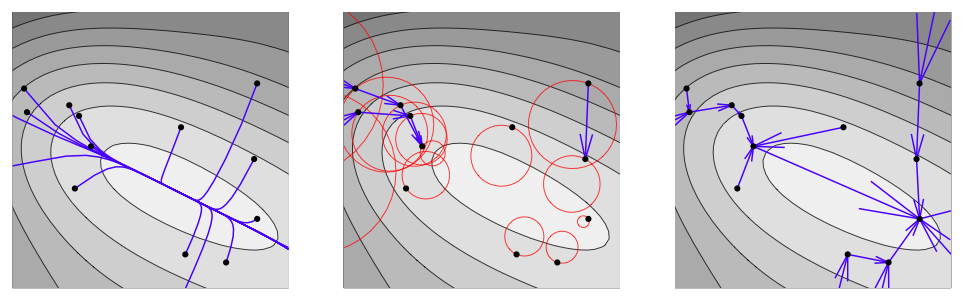
\includegraphics[width=0.9\textwidth]{MeanshiftMedianshiftQuickshift}
    \caption{Mean shift clustering (left) versus Median Shift clustering (center) versus Quickshift clustering (right) (Taken from Vedaldi \cite{vedaldi2008quick}.)}
    \label{fig:ms_qs}
\end{figure}

Quickshift clustering takes a slightly different approach, mainly used to speed up the clustering process \cite{vedaldi2008quick}. It does not model a global density estimate, but calculates the density for each data point. Next, for each point its neighbor with the highest density estimate (higher than its own) within a certain window is found. This results in a tree-like structure, where the data points at local density maxima become the head nodes, and define cluster and also its detection, the difference between mean-shift and quickshift is shown in Figure~\ref{fig:ms_qs}.

The window parameter $\tau$ in quickshift defines what range around each data point is used both to calculate its density estimate, and to look for data points available for clustering.

% subsubsection mode_finding_algorithms (end)

% subsection clustering_algorithms (end)

% section object_detection (end)
